\documentclass[a4paper]{article}
\usepackage[brazilian]{babel}
\usepackage[utf8]{inputenc}
\usepackage[T1]{fontenc}
\usepackage{listings}
\usepackage{pdfpages}
\usepackage{lscape}
\usepackage[titles]{tocloft} % Formatierung der Vezeichnisse

\newcommand{\cnpj}{12345678901234}
\newcommand{\senha}{senha123}
\newcommand{\nf}{\emph{plataforma} }
\newcommand{\erp}{\emph{erp} }
\newcommand{\dev}{desenvolvedor }

%Para sumário com linha pontilhada
\cftsetpnumwidth{1.0cm}
\renewcommand{\cftsecdotsep}{\cftdotsep}
\renewcommand{\cftsecleader}{\normalfont\cftdotfill{\cftsecdotsep}}

%opening
\title{NF\_V3}
\author{Fernando H. Crozetta}

\begin{document}

\maketitle

\begin{abstract}
Com a reescrita dos programas de comunicação com webservices do governo, foram alteradas as estruturas do projeto.

Por conta das grandes alterações, este documento serve como um guia para o \dev  que irá realizar a manutenção do fonte.
\end{abstract}
\pagebreak

{\def\makebox[#1][#2]#3{#3}%
	\tableofcontents % Inhaltsverzeichnis
}
\pagebreak
\section{Conceito}
A partir de versões anteriores de comunicação com webservices e diversos programas diferentes, que em essência realizam a mesma tarefa, foi pensada uma solução que pudesse atender a todas as chamadas de webservices do governo brasileiro, que utilizem o SOAP para comunicação.

Partindo do princípio de escrever uma vez, para que funcione em diversos programas, as rotinas foram modularizadas, e separadas em categorias, de acordo com sua natureza. Algumas permitem a chamada via linha de comando, outras são funções a serem chamadas apenas pelas interfaces, etc...

A partir da estrutura de diretórios de arquivos de configuração de clientes, foi redesenhada a forma de organizar estes arquivos.
Foi realizada uma separação entre dados e programas, permitindo uma fácil manutenção e atualização em clientes.

A partir desta versão, todo e qualquer caminho precisa ser parametrizado, permitindo a mudança de diretórios sempre que for necessário.\footnote{Esta alteração também permite a personalização de acordo com a infra estrutura do cliente}.

Após a separação entre dados e programas; e separação de cada tipo de programa dentro da plataforma, a organização fica simples para leitura.

O conjunto de programas que realizam as tarefas de comunicação, junto com suas ferramentas, estrutura de diretórios, arquivos temporários,etc. Serão chamados neste documento de \emph{plataforma}, para melhor entendimento.

O sistema foi criado para ser auxiliar e secundário. Ou seja, ele apenas faz a troca de mensagens entre o webservice, e um outro programa. Neste documento, o programa chamador também será referenciado como \emph{erp}, 

\section{Estruturação de Diretórios}
Por padrão, existem apenas dois diretórios principais:
\begin{enumerate}
	\item NF\_V3
	\item NF\_V3\_dados
\end{enumerate}
Sendo o primeiro para programas e o segundo para os dados dos clientes
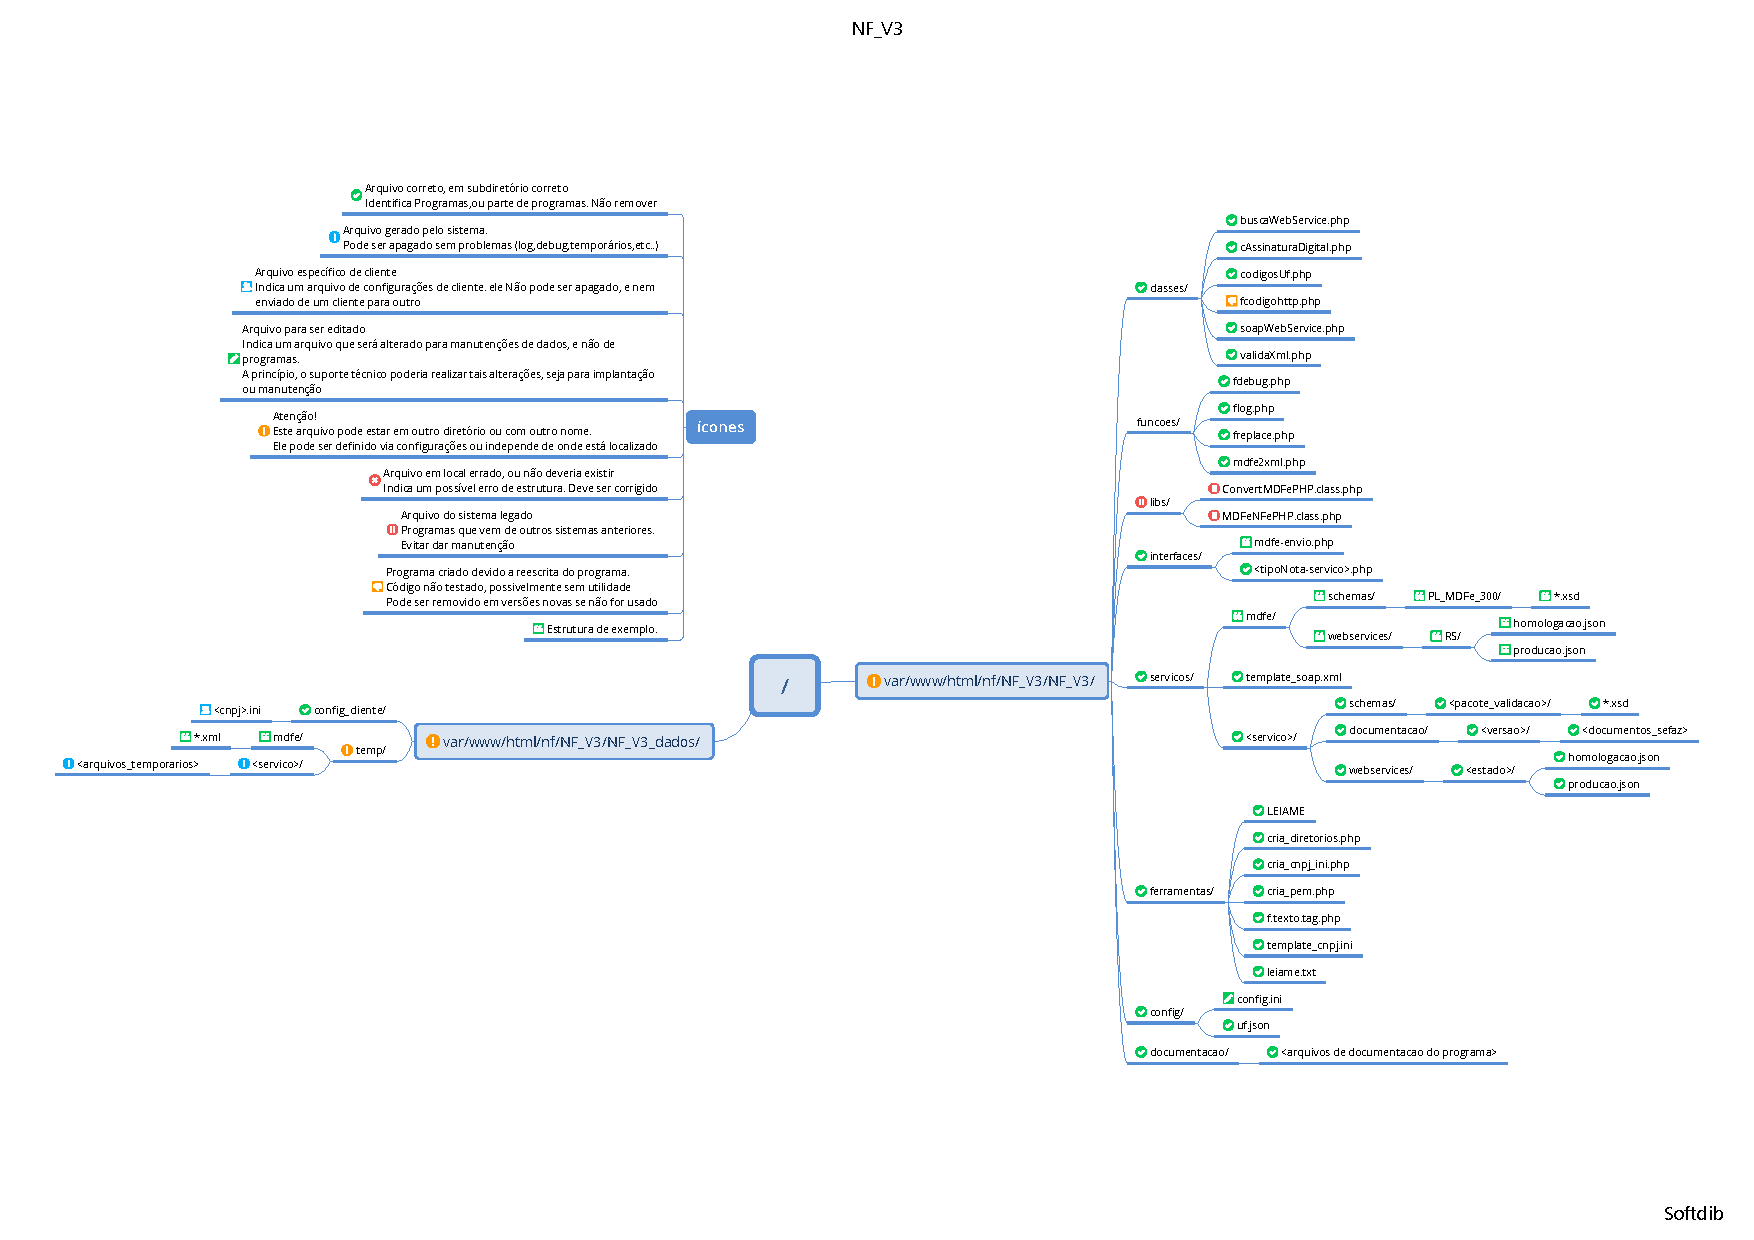
\includepdf[pages={-},fitpaper,rotateoversize]{mindmap.pdf}


\subsection{NF\_V3\_dados}
Dentro do diretório de dados do cliente temos, por padrão, um diretório \emph{config\_cliente}, e um diretório \emph{temp}, que servem para armazenas os dados persistentes e temporários de cada cliente.

\subsubsection{config\_cliente}
 Este diretório deve possui apenas arquivos de configuração de cada cnpj de empresa. Apesar do caminho padrão poder ser alterado, recomenda-se que sempre fique dentro do \emph{NF\_V3\_dados}. cada arquivo deve possui a seguinte nomenclatura:
 \begin{verbatim}
 <cnpj>.ini
 EX:12345678901234.ini
 \end{verbatim}
Dentro do arquivo, devem estar presentes, obrigatoriamente, os seguintes blocos de dados\footnote{os dados corresponde a uma empresa de cnpj \cnpj, cuja senha do certificado é \senha}:

\begin{lstlisting}
[empresa]
cnpj='12345678901234'

[certificado]
caminho_certificado="/var/www/html/nf/nfse/certificados/"
arquivo_certificado="/var/www/html/nf/nfse/certificados/12345678901234.pfx"
raiz_certificado='/var/www/html/nf/nfse/certificados/12345678901234'
senha="senha123"

[curl]
conexao_segura=S
verbose=0
porta=443
header=1
sslversion=3
ssl_verifyhost=0
ssl_verifypeer=0
connecttimeout=
timeout=
maxredirs=
followlocation=0
post=1
returntransfer=1
fresh_connect=0

[proxy]
servidor=
porta=00000
usuario=
senha=


[outros_dados]
cnpj="ERRO!Load de arquivo errado"
\end{lstlisting}
A princípio não há uma ordem obrigatória para os blocos de informação, entretanto, o bloco \emph{[outros\_dados]} deve ficar por último, pois caso o arquivo seja lido de forma errada, o cnpj trará uma mensagem de erro para o \dev.

Além dos dados obrigatórios, existem também os dados específicos de cada tipo de nota. Estes dados devem ser criados pelo \dev  da interface da \nf para o \erp.

Abaixo, um exemplo de um arquivo já preenchido com os dados de dois serviços:
\begin{lstlisting}
[empresa]
cnpj="12345678901234"

[certificado]
caminho_certificado="/var/www/html/nf/nfse/certificados/"
arquivo_certificado="/var/www/html/nf/nfse/certificados/12345678901234.pfx"
raiz_certificado='/var/www/html/nf/nfse/certificados/12345678901234'
senha="senha123"

[mdfe]
versao="3.00"
pacote="PL_MDFe_300"
versao_soap="2"
dir_retorno='/var/www/html/nf/NF_V3/NF_V3_dados/temp/mdfe/'

[nfse]
ip="e-gov.betha.com.br"
ambiente=2
url_producao="http://e-gov.betha.com.br/e-nota-contribuinte-ws/nfseWS?wsdl"
url_homologacao="http://e-gov.betha.com.br/e-nota-contribuinte-test-ws/nfseWS?wsdl"

[dnfe]
versao="1.01"
pacote="PL_NFeDistDFe_102"
versao_soap="2"
dir_retorno='/var/www/html/nf/NF_V3/NF_V3_dados/temp/dnfe/'
dir_procNFe='/user/nfe/12345678901234/DEST/'
dir_resEvento='/var/www/html/nf/NF_V3/NF_V3_dados/temp/dnfe/resEvento/'
dir_resNFe='/var/www/html/nf/NF_V3/NF_V3_dados/temp/dnfe/resNFe/'
dir_procEventoNFe='/var/www/html/nf/NF_V3/NF_V3_dados/temp/dnfe/procEventoNFe/'
dir_naoImplementado='/var/www/html/nf/NF_V3/NF_V3_dados/temp/dnfe/naoImplementado/'
dir_saida_cobol='/user/nfe/12345678901234/CaixaSaida/Sefaz/'

[curl]
conexao_segura=S
verbose=0
porta=443
header=1
sslversion=3
ssl_verifyhost=0
ssl_verifypeer=0
connecttimeout=
timeout=
maxredirs=
followlocation=0
post=1
returntransfer=1
fresh_connect=0

[proxy]
servidor=
porta=00000
usuario=
senha=


[outros_dados]
cnpj="ERRO!Load de arquivo errado"
\end{lstlisting}

\subsubsection{temp}
O diretório temp identifica o diretório de trabalho da \nf. Este diretório \emph{NÃO} pode ficar dentro do diretório de programas, pois corre o risco de ser atualizado em clientes.

Dentro deste diretório se encontram subdiretórios referentes ao servido de nota buscado: \emph{temp/mdfe} e \emph{temp/dnfe}, por exemplo.

Tudo o que estiver sob o diretório temp pode ser apagado, sem exceção. Por este motivo, tudo o que for necessário ser salvo, deve ser colocado em parâmetros dentro do config do cliente pelo \dev.

\subsection{NF\_V3}
Este diretório possui os programas e binários para a execução das rotinas de comunicação entre os webservices e o \erp.

Os arquivos devem seguir os padrões de desenvolvimento definidas no diretório de documentação, e de acordo com os arquivos LEIAME, dentro do próprio diretório. Nos comentários do cabeçalho do programa, deve conter :
\begin{enumerate}
	\item identificação do autor
	\item data
	\item descrição do programa
	\item modo de uso (caso seja chamado via linha de comando)
\end{enumerate}

Os programas foram separados em diretórios, que identificam sua função, e modos de uso:
\begin{enumerate}
	\item interfaces
	\item classes
	\item funcoes
	\item ferramentas
	\item libs
	\item servicos
	\item config
	\item documentacao
\end{enumerate}
\subsubsection{interfaces}
Neste diretório, e apenas neste diretório, se localizam os programas a serem chamados pelo \erp.
Até o presente momento, é preciso realizar o comando \emph{cd /caminho/para/interfaces/} e depois executar o comando php\footnote{Este é um bug conehcido e está na lista para correções}.

A nomenclatura de todos os programas aqui criados é:
\begin{lstlisting}
<tipo de nota>-<servico>.php
EX:mdfe-consulta.php
\end{lstlisting}
Essa nomenclatura facilita para a localização dos serviços de cada tipo de nota

\subsubsection{classes}
Neste diretório devem ficar apenas as classes que são chamadas pelas interfaces e ferramentas. Nenhum programa deste diretório deve ser chamado por linha de comando.

\subsubsection{funcoes}
Neste diretório, os programas devem possuir apenas uma função dentro dele. Estes arquivos adicionam uma funcionalidade simples aos programas, servindo como apoio para o \dev que esta realizando a manutenção no código. Ele pode ser incluído nas interfaces com o comando \emph{require\_once()} 

\subsubsection{ferramentas}
Os arquivos que estão aqui, não são necessariamente para uso interno da \nf, mas permitem que o \dev e suporte técnico possam executar algumas tarefas que podem ser necessárias. Elas são funções complementares, e tem como objetivo auxiliar primariamente o suporte técnico a resolver possíveis problemas.
\subsubsection{libs}
Os programas deste diretório são programas legado que foram alterados apenas para que funcionem com diretórios locais. Nenhuma alteração de código foi realizada. 

O \dev deve evitar realizar alterações nos programas deste diretório. Em teoria, este diretório ficará vazio com o passar do tempo.

\subsubsection{servicos}
Dentro deste diretório está localizada a estrutura de dados referentes aos webservices. Dentro dele estão os tipos de nota, separados por diretório; seguido de subdiretórios de schemas de validação, documentação proveniente da sefaz \footnote{Caso seja necessário adicionar documentação do \erp, separar os diretórios.}, e webservices. Este último, por sua vez é dividido em estados, e dentro de cada diretório de estado, existem dois arquivos:
\begin{enumerate}
	\item homologacao.json
	\item producao.json
\end{enumerate}
Estes dois arquivos contém a estrutura necessária para envio de dados e montagem de xml

\subsubsection{config}
Neste diretório se encontram os arquivos de configuração do programa. O primeiro arquivo é uf.json, que possui os código de cada estado brasileiro e seu código IBGE. O segundo é config.ini, que possui os direcionamentos de caminhos para log, debug, servicos dos webservices, temp e diretório de dados(NF\_V3\_dados). Estes arquivos só precisam ser alterados se for necessária uma alteração grande nas estruturas do \nf.

\subsubsection{documentacao}
Este diretório deve possuir a documentação referente a \nf, sem conter manuais da sefaz e outros arquivos que não dizem respeito a construção e manutenção desta \nf.

\section{Desenvolvimento: classes/}

\subsection{buscaWebService.php}
Classe que busca os dados de webservice com base no tipo de nota solicitado, estado, ambiente, e serviço. 
Esta classe foi reescrita para buscar dados de arquivos json, ao invés de xml, como nas versões legado do programa.
Instanciação de classe:
\begin{lstlisting}[language=Php]
require_once("../classes/buscaWebService.php");
$var = BuscaWebService(($uf,$tipo_nota,$tipo_ambiente);
\end{lstlisting}
\subsubsection{construtor}
\begin{lstlisting}[language=Php]
function __construct($uf,$tipo_nota,$tipo_ambiente='homologacao')
\end{lstlisting}
\begin{itemize}
	\item uf: Sigla do estado do webservice.Maiúsculo.
	\item tipo\_nota: Tipo de nota a ser usada.EX:mdfe,dnfe,nfe,etc.Minúsculo.
	\item tipo\_ambiente: string:homologacao/producao. homologacao, caso não seja passado o parâmetro
\end{itemize}
\subsubsection{buscarServico}
\begin{lstlisting}[language=Php]
$var->buscarServico($nome_servico,$versao);
\end{lstlisting}
\begin{itemize}
	\item nome\_servico: Servico do tipo de nota, definido pelo \dev\footnote{Este nome é a chave dentro do arquivo de webservices}.
	\item versao: Versão do serviço buscado, definido pelo \dev no config do cliente
\end{itemize}
Retorna um objeto com os dados do webservice buscado


\subsection{CAssinaturaDigital.php}
Classe alterada a partir do fonte legado. As alterações foram realizadas apenas para suportar a nova estrutura.
A lógica do programa não foi alterada.
Instanciação da classe:
\begin{lstlisting}[language=Php]
require_once("../classes/CAssinaturaDigital.php");
$var = new CAssinaturaDigital($arquivo,$cnpj);
\end{lstlisting}
\subsubsection{construtor}
\begin{lstlisting}[language=Php]
function __construct($arquivo_xml,$cnpj)
\end{lstlisting}
\begin{itemize}
	\item arquivo\_xml: caminho e nome do arquivo xml a ser assinado
	\item cnpj: cnpj do emissor do xml
\end{itemize}
\subsubsection{getXml}
Não possui parâmetros.
Retorna o xml lido no construtor
\subsubsection{getErro}
Não possui parâmetros.
Retorna a string de erros.
Evitar usar esta função.Ela vem do fonte legado.
\subsubsection{salvar}
\begin{lstlisting}
public function salvar($destino='')
\end{lstlisting}
\begin{itemize}
	\item destino: caminho e nome do arquivo de saída. Caso não seja passado, será sobreescrito no arquivo original
\end{itemize}
Uso:
\begin{lstlisting}
$var->salvar($destino);
\end{lstlisting}
\subsubsection{assinarXml}
Esta função vem do legado, e por padrão recebe dois parâmetros, mas a princípio a softdib está usando apenas a primeira tag.
\begin{lstlisting}
content...
\end{lstlisting}







\end{document}
